With the recent shift of application architectures from monolithic to containers and microservices, serverless computing has risen as a promising cloud service where simple, stateless, 
event-driven functions comprise applications and services. 
%It represents a revolutionary programming and deployment paradigm known as Function as a Service (FaaS). 
Serverless platforms relieve
developers of the burden of provisioning servers to deploy 
cloud and web applications.
Programmers typically write functions in high-level languages which are triggered by the platform in response to events from external sources or other cloud services. 

This function-level abstraction also provides fine-grained computational resource isolation and usage, meaning that each serverless function can autoscale independently based on the rate of incoming events. Providing such elasticity helps avoid a single point failure and performance bottlenecks in data-intensive application. From this perspective, serverless architecture is an ideal system for machine learning applications, especially for online training~\cite{ref:online} and inference, which transfer and manipulate large amounts of data or for 
which the input sizes vary.

To enable such an event-driven system, one concerning situation is for machine learning applications that receive their data from  heterogeneous IoT devices, ranging from temperature sensors to mobile phones to autonomous drones. For such deployments, application execution should be ``near'' (in terms of network latency) the data sources to achieve fast response times. Such settings motivate us to explore extending the serverless model to the edge for execution of data analytics applications.

One challenge with edge computing is the scarcity of computational resources relative to resource rich public and private clouds.  Moreover, public/private clouds may offer specialized hardware (e.g. GPUs) that significantly speed up machine learning applications, which is not commonly available in resource-restricted edge clouds.
In our work, we investigate how to extend the serverless computing model to hybrid cloud systems that consist of edge and cloud resources and that integrate GPU acceleration. 

\begin{figure}
    \centering
    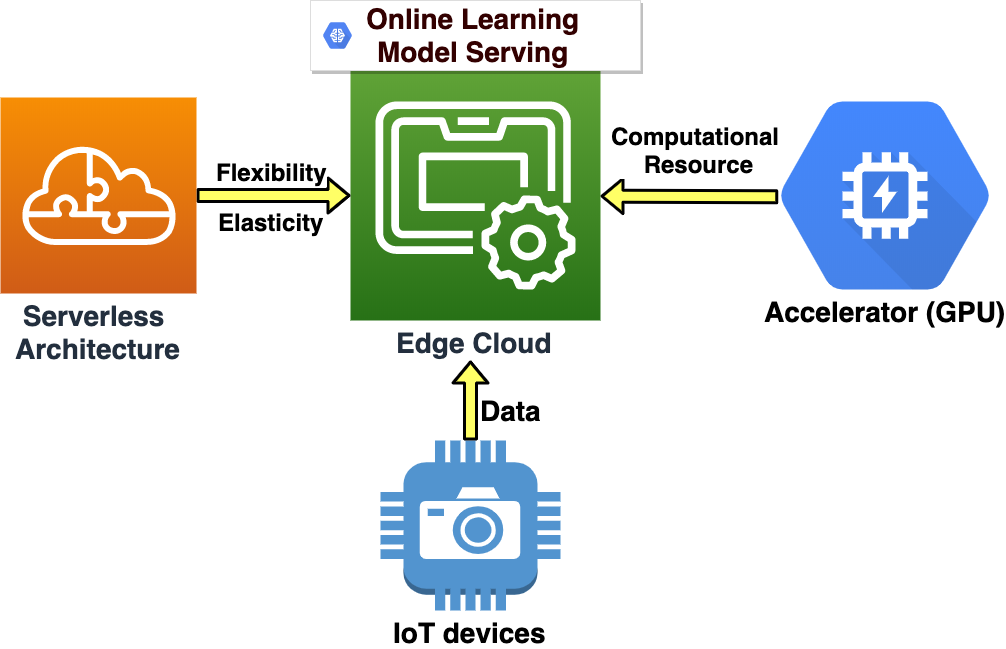
\includegraphics[scale=0.25]{figures/edge}
    \caption{The abstract design of STOIC -- a system for executing distributed machine learning applications in IoT (e.g. edge + cloud) settings.
\label{fig:edge}}
\end{figure}

Toward this end, we present STOIC -- a Serverless TeleOperable Hybrid Cloud. As depicted in Figure~\ref{fig:edge}, STOIC is a framework to which IoT devices stream data in batches for training and inference by machine learning applications.  The framework implements serverless computing and deployment for the applications. Unique to STOIC, however, is its scheduling system which intelligently places the application workload on edge and cloud systems that it predicts will result in the fastest time to completion. Moreover, STOIC takes advantage of GPU acceleration when available from the underlying cloud resource. In this paper, we discuss the design and implementation of this architecture, investigate the efficacy of using this extended serverless model for machine learning applications that span edge-cloud systems, and  empirically evaluate the performance of doing so. Using real workloads and deployments, we find that STOIC reduces the total response time of the applications we study from 6.48\% to 32.05\%, compared with four different runtimes, each running in isolation. Finally, we discuss related and future work and conclude.
